\section{Extensions and the limits of each conclusion}\label{sec:mech}

\paragraph{In brief.}
How much storage protects a parasite depends on how it waits, survives, and meets its hosts. Each of these is examined separately below, with exact results where available and small-noise comparisons elsewhere. A long sheltered stage does not guarantee protection when waiting deaths, linked host fluctuations, or host absences change the comparison.

An additional host can alter transmission success, waiting times, and the environments encountered by descendants. These comparisons test where the storage argument of \citet{dobson2020} holds. Loss of reproduction remains distinct from extinction of a finite population.

Unless stated otherwise, the baseline fixes rates at their arithmetic means. Rings are calibrated to that threshold, counting one birth per circuit. We write \(D_2=\sigma^2K\) for quadratic loss. In route networks, \(\Delta\) is the log multiplier on specified reproductive returns that restores zero growth, so loss depends on the birth convention (Section~\ref{sec:model}). Examples are illustrative. Proofs are in Appendix~\ref{app:mech}; ``refereed'' denotes the internal review described in Section~\ref{sec:model}.

\subsection{Scarcity that delays transmission}
The original ring loses individuals that leave but fail to transfer. In a contact-limited stage, host scarcity instead prolongs waiting, during which individuals can die. Let the death probability be \(\mu\), encounter probability \(ch_t\), and yield per encounter \(b_j\), where \(\mathbb E h_t=1\). Then
\begin{equation}\label{eq:mech-contact-model}
 s_j(t)=1-\mu-ch_t,\qquad g_j(t)=b_jch_t,
 \qquad d=\frac{\mu}{\mu+c}.
\end{equation}
The constraint \(\mu+ch_t\leq1\) excludes an unbounded lognormal host for every \(c>0\). The death fraction \(d\) applies at the constant-mean-host threshold, and need not match the fraction under correlated fluctuations.

\begin{proposition}[Contact limitation]\label{prop:mech-contact}
Let the mean ring be primitive, with positive transfers and positive baseline staying in stage \(j\). Let \(h_t=1+\sigma\xi_t\), where \(\xi\) is bounded, stationary ergodic, centered, has unit variance, and has covariance \(\phi^{|\ell|}\), \(-1<\phi<1\). Keep every changed contribution positive for sufficiently small \(|\sigma|\). Put
\begin{equation}\label{eq:mech-contact}
 \theta=\frac{\phi}{1-\phi},\quad q_k=\frac{\phi}{\phi+(1-\phi)\tau_k},\quad
 R=\prod_kq_k,\quad K_g=\frac{1+2\theta}{2\mathcal T}-\frac{R}{1-R}.
\end{equation}
At \(\phi=0\), set \(q_k=R=0\). Then
\begin{equation}\label{eq:mech-contact-coefficient}
 D_2=\sigma^2K_c,\qquad K_c=d^2K_g+d(1-d)\frac{q_j-R}{1-R}.
\end{equation}
The remainder is \(O(|\sigma|^3)\), or \(O(\sigma^4)\) if the whole driver process is invariant under sign reversal. For \(0\leq\phi<1\) and \(0<d\leq1\), \(K_c>0\). At \(d=0\), reproductive value is conserved and \(D=0\) at every admissible amplitude. The value \(d=1\) denotes the gain-only perturbation, with the staying perturbation omitted. If a different steady stay tends to infinity with the other stays, \(d\), and memory fixed, then
\begin{equation}\label{eq:mech-contact-limit}
 \lim K_c=d(1-d)q_j.
\end{equation}
\end{proposition}
The coefficient was proved and refereed; its bounded-forcing remainder is derived separately in Appendix~\ref{app:mech-contact}. Without memory, contact limitation multiplies the gain-only coefficient by \(d^2\). Positivity fails with negative memory, and the long-stay value is a limit, not a floor (Fig.~\ref{fig:mech-1}; details in Online Resource 1). The continuous-time expansion replaces \((1+2\theta)/(2\mathcal T)\) by \(\theta/\mathcal T\), so the discrete no-memory factor does not extend to a rapidly changing continuous-time host. Storage therefore depends on mortality while awaiting transmission.

\begin{figure}\centering
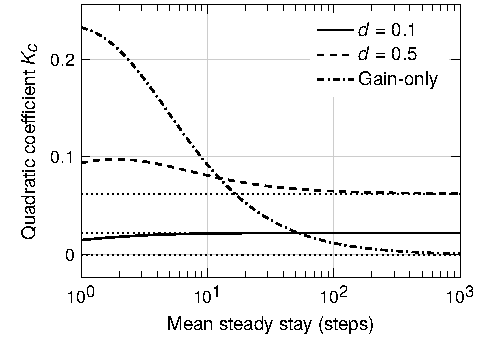
\includegraphics[width=84mm]{figures/mech-1.pdf}
\caption{Contact-limited quadratic loss coefficient against the mean steady stay, with contact stay three and memory \(\phi=0.5\). Solid, dashed, and dash-dotted curves denote \(d=0.1\), \(d=0.5\), and gain-only transmission. Dotted horizontal lines mark the corresponding long-stay limits, including zero for gain-only transmission. These are coefficients of host variance, not finite-noise losses}\label{fig:mech-1}
\end{figure}

\subsection{The distribution of time spent in a stage}
Equal mean stays need not provide equal protection. A sheltered segment has a kernel (expected output at each lag after entry, including survival and reproduction). Equal kernels and unchanged exposed dynamics preserve the growth exponent and threshold, regardless of compartment names. Dividing a stay generally changes its kernel \citep{blythe1984,lloyd2001}.

\begin{proposition}[Renewal time and stay shape]\label{prop:mech-renewal}
Consider a finite primitive reference model at the mean-rate threshold, with the marked regenerative transfer as the sole counted birth. Its frequency is \(b=1/\mathcal T\). Here \(K\) denotes the coefficient of the restoring multiplier \(\Delta\), equal to \(D_2/\sigma^2\) in a ring with one counted birth per circuit. All rates are constant except that transfer, multiplied by \(\exp(\sigma\xi_t-\sigma^2/2)\), with centered stationary unit-variance Gaussian AR(1) driver, \(0\leq\phi<1\). Assume the local perturbation expansion applies. Let \(L\) be the positive integer return time between uses of that event by the reference lineage, \(\mathcal T=\mathbb E L\), and \(R=\mathbb E[\phi^L]\). Then
\begin{equation}\label{eq:mech-renewal}
 K=\frac{1+2\theta}{2\mathcal T}-\frac{R}{1-R},\qquad
 K<0\ \Longleftrightarrow\ R>\frac{1+2\theta}{1+2\theta+2\mathcal T}.
\end{equation}
At fixed \(\mathcal T\) and \(0<\phi<1\), a mean-preserving spread in convex order lowers \(K\). For a death-free steady stay of mean \(b\) represented by \(m\) equal geometric substages, integer \(1\leq m\leq b\), its transform is \((1+b/(m\theta))^{-m}\). Increasing \(m\) strictly raises \(K\) when \(\phi>0\), provided all compared models remain primitive. At \(\phi=0\), \(K=1/(2\mathcal T)\). A sum of geometric stays cannot satisfy the gain condition.
\end{proposition}
This result was proved and refereed. The return-time transform, rather than variance alone, orders the coefficients. Rare long returns can give \(K<0\), while a fixed sheltered delay after a geometric exposed stay of mean \(a>1\) makes \(K\to0\) at fixed memory. Neither conclusion locates a finite-noise threshold. Worked examples are in Online Resource 1. Mortality during a fixed delay incurs its full survival cost (Lemma~\ref{lem:mech-mortality}).

\begin{proposition}[Every stay fixed]\label{prop:mech-fixed}
Suppose every stay is fixed, the cycle has \(n\) time positions, and one transfer has a positive stationary multiplier \(h\) with \(\mathbb E|\log h|<\infty\). If the environment is ergodic under the shift by \(n\) steps, then \(D=-\mathbb E\log h\). In particular, for the mean-one lognormal multiplier, \(D=\sigma^2/2\), regardless of the fixed durations.
\end{proposition}
This separate cohort proof was refereed. An all-fixed cycle with \(n>1\) is not primitive, so the preceding expansion cannot be substituted there. Both mean duration and its spread matter (Fig.~\ref{fig:mech-4}).

\begin{figure}\centering
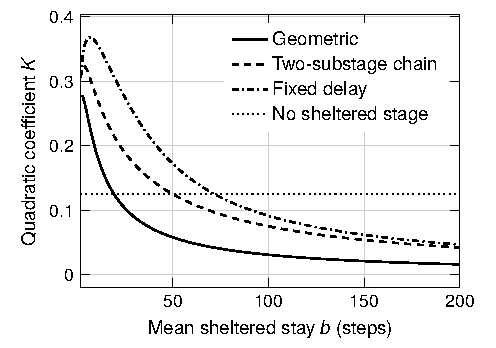
\includegraphics[width=84mm]{figures/mech-4.pdf}
\caption{Quadratic loss coefficients for a geometric exposed stay of four steps and a sheltered stay of mean \(b\), at \(\phi=0.9\). Solid, dashed, and dash-dotted curves give a geometric sheltered stay, two equal geometric substages, and a fixed delay. The dotted horizontal line gives the no-sheltered-stage coefficient. Fixed delays are evaluated at integer steps, and the exposed stay remains random in every comparison}\label{fig:mech-4}
\end{figure}

\subsection{Temperature-dependent completion and development}
Temperature affects development and death, requiring joint treatment of staying and transfer. Physical shelter from temperature differs from buffering host abundance \citep{kutz2014,aleuy2020}. 

Changing stage-leaving speed (the developmental clock) alone leaves the threshold unchanged when completion probabilities (successful completion among leavers) are constant; joint thermal changes in both can alter the quadratic sign (Proposition~\ref{prop:mech-thermal}, Appendix~\ref{app:mech}).
These statements were proved and refereed. Conservation requires constant completion probabilities in every exposed stage. A clock-sensitive stage remains exposed when another stage has temperature-dependent completion. No finite-amplitude remainder bound is supplied; an illustrative numerical comparison is in Online Resource 1.

When staying rates fluctuate, their logarithmic penalties also enter the bound, weighted by time spent staying (Proposition~\ref{prop:mech-edge-bound}, Appendix~\ref{app:mech}).
This bound was proved and refereed. A temperature-sensitive reservoir must be evaluated through both completion and staying rates (worked example in Online Resource 1).

\subsection{Encounter functions and alternative routes}
Curved encounter functions of host abundance $H$ change both mean transmission at fixed mean host abundance and the quadratic fluctuation response (Proposition~\ref{prop:mech-curvature}, Appendix~\ref{app:mech}).
The derivation was reproduced independently. Smoothness at the mean alone does not imply the required expectation or growth expansion. A saturating type-II encounter cannot give a quadratic benefit when \(K_g\geq0\), whereas an inverse response does so when \(K_g<1\). Bounds concern the rate's logarithmic gap, which for a normalized power \(H^\eta\) (elasticity \(\eta\)) is \(\eta^2\sigma^2/2\).

\begin{proposition}[Alternative, optional, and bypass routes]\label{prop:mech-routes}
Assume every compared mean model is primitive on retained states, calibrated to its own threshold, with fixed staying and the stated mean-one Gaussian AR drivers. In a parallel network, a central stage of stay \(\tau_0\) enters host \(j\) with reproductive share \(w_j\geq0\), \(\sum_jw_j=1\), and host stay \(\tau_j\). Count all returns as births. Without memory, put \(\mathcal T=\tau_0+\sum_jw_j\tau_j\), \(u_j=w_j\kappa_j\), and \(V=\mathbf u^{\mathsf T}\mathbf C\mathbf u\), with \(\mathbf C\) the log-driver correlation matrix. Then
\begin{equation}\label{eq:mech-parallel}
 \Delta_2=\frac{\sigma^2V}{2\mathcal T}.
\end{equation}
A newcomer of share \(0<f\leq1\), variance coefficient \(U\), covariance \(C\) with the old aggregate, and stay difference \(\delta\tau\) lowers this coefficient exactly when
\begin{equation}\label{eq:mech-newcomer}
 f\mathcal T(V-2C+U)<2\mathcal T(V-C)+V\delta\tau.
\end{equation}
For a fraction \(0\leq f\leq1\) using an optional steady host of survival \(0\leq q\leq1\), define \(Y=1-f+fq\), require \(Y>0\), and put \(\alpha=fq/Y\). At equal mean reproduction, \(\mathcal T=\tau_0+\tau_1+\alpha\tau_p\), \(R=q_0q_1(1-\alpha+\alpha q_p)\), and \(K_{\rm opt}\) is \eqref{eq:mech-renewal}. For a bypass of relative yield \(q\geq0\), again with \(0\leq f\leq1\) and \(Y>0\), put \(\alpha=(1-f)/Y\), \(\mathcal T=\tau_0+\alpha\tau_1\), and \(R=q_0(1-\alpha+\alpha q_1)\). Then
\begin{equation}\label{eq:mech-bypass}
 K_{\rm by}=\alpha^2\left[\frac{1+2\theta}{2\mathcal T}-\frac{q_0q_1}{1-R}\right].
\end{equation}
For either route, the exact advantage at fixed other rates is \(\log Y+\Delta_{\rm base}-\Delta_{\rm route}\).
\end{proposition}
These formulas were reproduced independently. Independent alternatives enter through shares squared, whereas independent obligatory transfers add their quadratic terms on the same mean matrix. A noisy newcomer can increase loss. An optional host with \(fq>0\) lowers the no-memory coefficient at equal mean reproduction, but this benefit fails under strict alternation (examples in Online Resource 1). For a single noisy transfer and two equal stays \(a>1\),
\begin{equation}\label{eq:mech-negative-memory}
 K_g=\frac{1}{4a}\frac{1+\phi(1+2/a)}{1-\phi(1-2/a)}<0
 \quad\Longleftrightarrow\quad \phi<-\frac{a}{a+2}.
\end{equation}
Temporal independence therefore cannot be replaced by a variance condition. A strict-alternation example is in Online Resource 1. Relapse also permits gains, as in \citet{white2016}; its continuous-time renewal criterion is in Appendix~\ref{app:mech-renewal}.

\subsection{One host on two transfers and linked hosts}
Transfers responding to the same host or to linked hosts depend on covariances at directed time lags, beyond same-day correlations \citep{tuljapurkar1982a,tuljapurkar2006}. Define
\(\rho_{ij}(\ell)=\mathbb E[\xi_i(t)\xi_j(t-\ell)]\): host \(i\) is observed later. Both transfers read their hosts at the current step.

\begin{proposition}[Linked transfers]\label{prop:mech-linked}
Let a primitive fixed-staying ring at threshold have lognormal transfer multipliers driven by a stable finite-dimensional Gaussian autoregression, or a finite-dimensional Gaussian linear extension of it, centered with unit marginal variances and with the local expansion justified. For transfer sensitivities \(\kappa_i\), let \(u_{j\to i}(\ell)\) be the reference probability of using transfer \(i\) at lag \(\ell\) after transfer \(j\). Then
\begin{equation}\label{eq:mech-linked}
 K=\sum_{i,j}\kappa_i\kappa_j\left[\frac{\rho_{ij}(0)}{2\mathcal T}
 +\sum_{\ell\geq1}\rho_{ij}(\ell)\left(\frac1{\mathcal T}-u_{j\to i}(\ell)\right)\right].
\end{equation}
For two hosts write \(K=K_1+K_2+X\). A net quadratic gain requires \(X<-(K_1+K_2)\), and adding the second host helps relative to the first alone exactly when \(X<-K_2\). For unit sensitivities, exchanging hosts gives
\begin{equation}\label{eq:mech-order}
 K_{12}-K_{21}=-\sum_{\ell\geq1}[\rho_{21}(\ell)-\rho_{12}(\ell)]
 [u_{1\to2}(\ell)-u_{2\to1}(\ell)].
\end{equation}
\end{proposition}
The formulas and specified simulations were reproduced independently. Reversing linked hosts changed the sign of finite-noise loss in the illustrative example (Fig.~\ref{fig:mech-3}; details in Online Resource 1). Reversible cross-covariances or identical directed return distributions eliminate the quadratic order effect; equal mean travel times alone do not.

For one host driving both transfers of a two-stage ring with stays \(a,b\), the same-sign coefficient is
\begin{equation}\label{eq:mech-common}
 K_+=\frac{2ab+\theta[2(a+b)-(a-b)^2]}{(a+b)[ab+\theta(a+b)]}.
\end{equation}
For \(0\leq\phi<1\), it is negative exactly when \((a-b)^2>2(a+b)\) and \(\theta>2ab/[(a-b)^2-2(a+b)]\). At equal stays it is \(1/a>0\). Continuous time lacks the instantaneous cost \((\kappa_1+\kappa_2)^2/(2\mathcal T)\), so equal same-sign sensitivities give a gain for any unequal pair of leaving rates there. Shrinking the time step reconciles the formulas (Appendix~\ref{app:mech-common}). This distinction also matters when interpreting switching host--vector models \citep{watts2021}. Linked hosts can preserve a useful ordering of encounters, but correlation does not supply an unconditional benefit.

\begin{figure}\centering
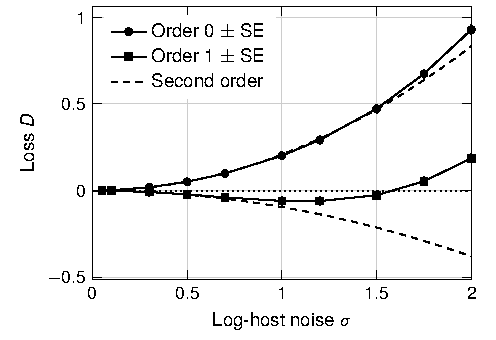
\includegraphics[width=84mm]{figures/mech-3.pdf}
\caption{Loss against log-host noise for two orders of linked hosts on a ring with stays \((5,50,5)\). Circles denote host 1 on transfer 0 and host 2 on transfer 1, squares the reverse order. The host autoregression has radius 0.9 and rotation angle \(\pi/10\). Solid lines join simulation estimates, bars give one standard error, and dashed curves are the respective quadratic predictions. The horizontal dotted line marks zero loss. Transfer 2 is steady}\label{fig:mech-3}
\end{figure}

\subsection{Hosts that can be absent}\label{subsec:mech-absent}
Host absence violates assumption A13. Period-two outages explain the mechanism behind 51 stay reversals in replayed \textit{Tribolium} larval records (Section~\ref{sec:num}).
Here \(a,s\) are finite mean stays, with \(a>1,s\geq1\). Set
\begin{equation}\label{eq:mech-outage-model}
 b=1/a,\quad p=1-b,\quad \varepsilon=1/s,\quad q=1-\varepsilon,
 \qquad \mathbf A_t(c)=\begin{pmatrix}p&\varepsilon c\\b h_t&q\end{pmatrix},\quad c>0.
\end{equation}
The restoring loss is \(D=\log c_*\), where the top matrix growth exponent vanishes at \(c_*\).

\begin{proposition}[Thresholds with absent hosts]\label{prop:mech-outage}
Let \(h_t\geq0\) be stationary ergodic with \(\mathbb E h_t=1\). The threshold exists uniquely and is finite. Temporal independence gives \(D\geq0\). For \(h=(2,0)\) repeated with uniform random phase,
\begin{equation}\label{eq:mech-outage-alt}
 D=\log\frac{(2a-1)(2s-1)}{2((2a-1)s-a+1)}<0,\qquad
 D_s=\frac{1}{(2s-1)((2a-1)s-a+1)}>0.
\end{equation}
If \(\mathbb E h_t^4<\infty\), then, at fixed \(a\) and host law,
\begin{equation}\label{eq:mech-outage-long}
 D=\frac{A}{s}+O(s^{-2}),\qquad
 A=\frac{\operatorname{Var}(h_t)}2+
 \sum_{\ell\geq1}p^{\ell-1}\operatorname{Cov}(h_t,h_{t-\ell}).
\end{equation}
For \(A\ne0\), every fixed \(\kappa>1\) eventually gives
\(\operatorname{sign}[D(a,\kappa s)-D(a,s)]=-\operatorname{sign}A\).
If additionally \(h_t\leq M<\infty\), put \(R=b/(256M^2)\). Then
\begin{equation}\label{eq:mech-outage-sign}
 \operatorname{sign}D_s=-\operatorname{sign}A,\quad
 \operatorname{sign}D=\operatorname{sign}A
 \quad\text{when}\quad
 0<s^{-1}<\min\{R/2,|A|R^2/4\},\quad A\ne0.
\end{equation}
\end{proposition}

With some staying, a finite threshold bound can remain available even when a host is sometimes absent (Proposition~\ref{prop:mech-outage-bound}, Appendix~\ref{app:mech}).
Propositions~\ref{prop:mech-outage} and~\ref{prop:mech-outage-bound} are proved in Appendix~\ref{app:mech-outage} and checked independently. The derivative sign under fourth moments alone remains open. Negative \(A\) shows how longer storage can remove an advantage of alternating host access.

\subsection{Dispersal among patches}
Dispersal changes the host histories encountered by descendants across patches. For the Gaussian host laws and island movement in Proposition~\ref{prop:mech-dispersal}, this can yield a quadratic gain, written $D_2=\sigma^2F<0$, where $F$ is the spatial loss coefficient (Appendix~\ref{app:mech}).
The coefficient was reproduced independently. Simulated gains ended at larger tested amplitudes (Fig.~\ref{fig:mech-2}; details in Online Resource 1). These sampled signs do not establish an interval theorem.

A long steady stage can also remove part of the spatial gain. Its coefficient and sign condition are in Appendix~\ref{app:mech-spatial}. The logarithmic-gap bound survives movement, transit losses, and unequal patch quality when these are included in the baseline. Perfectly synchronous hosts with conservative movement give exactly the aggregate single-patch ring. Movement therefore helps through differing environmental histories; effective variance replacement applies only in restricted small-noise cases.

\begin{figure}\centering
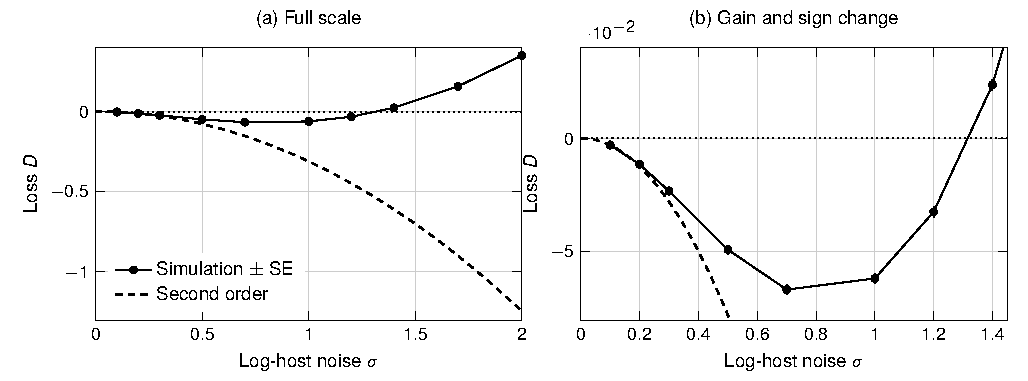
\includegraphics[width=174mm]{figures/mech-2.pdf}
\caption{Dispersal loss for stays \((2,2)\), four independent island patches, movement fraction 0.15 in stage 1, and memory \(\phi=0.8\). Circles joined by a solid line are estimates from random matrix products, bars give one standard error, and the dashed curve is \(\sigma^2F\). Panel (a) shows the full scale and panel (b) enlarges the gain and sign change. The horizontal dotted line marks zero loss. Movement follows demography, and there is no transit mortality}\label{fig:mech-2}
\end{figure}

\subsection{The mechanisms together}
The R16 numerical study combined contact limitation, regularized stays, alternative hosts, asynchronous patches, and storage mortality. It used a bounded two-state host, three illustrative cycles, and two step sizes, with 192 admissible cells. Independent reproduction covered selected cells and all comparison counts. All 18 resolved gains involved patches. Quadratic predictions sometimes had the wrong sign. This comparison combines finite amplitude with a skewed host law outside the standardized small-amplitude family, and has no comparator without a long stage. Details are in Online Resource 1; extinction comparisons and the calibration limitation are in Appendix~\ref{app:mech-r16}.

Table~\ref{tab:mech-summary} collects the model changes and their domains.

\begin{table}[htbp]\centering\scriptsize
\setlength{\tabcolsep}{2pt}
\caption{Summary of the changed models. M denotes arithmetic-mean rates, H constant mean host abundance, and T constant mean temperature. Loss is dimensionless log reproduction per circuit or specified birth. Q denotes quadratic, E exact, and N numerical results. R denotes internal proof review, I independent numerical reproduction, and O one derivation or study. Complete hypotheses are in the cited results, including primitivity for local expansions. Illustrative examples are in Online Resource 1}\label{tab:mech-summary}
\begin{tabular*}{\textwidth}{@{\extracolsep{\fill}}p{0.18\textwidth}p{0.06\textwidth}p{0.09\textwidth}p{0.07\textwidth}p{0.42\textwidth}p{0.08\textwidth}@{}}\toprule
Changed model & Base & Units & Order & Condition & Status\\\midrule
Contact-limited transfer & M & circuit & Q & Proposition~\ref{prop:mech-contact}, \(0\leq\phi<1,d>0\): positive & R\\
Contact, long steady stay & M & circuit & Q & Fixed other stays and memory, limit \(d(1-d)q_j\) & R\\
No waiting deaths & M & circuit & E & Valid threshold contact model, conserved positive value & R/I\\
Renewal stay shape & M & circuit & Q & Proposition~\ref{prop:mech-renewal}, gain iff transform exceeds its threshold & R\\
Fixed delay with random stay & M & circuit & Q/N & \(a>1\), fixed \(0\leq\phi<1\); small noise before long delay & R\\
Every stay fixed & M & circuit & E & Integrable log, ergodic cycle-length shift & R\\
Mortality during storage & M & circuit & Q & Lemma~\ref{lem:mech-mortality}: one noisy transfer, independent environments, survival \(\exp(-\mu)\) per step & R\\
Thermal clocks & M/T & circuit & E/Q & Proposition~\ref{prop:mech-thermal}; conservation needs all completion probabilities constant & R\\
Thermal curvature & T & circuit & Q & Inequality~\eqref{eq:mech-thermal-curvature}, regularity and cross terms retained & R\\
Changing staying edges & M & circuit & E & Proposition~\ref{prop:mech-edge-bound}, finite logs and existing threshold & R\\
Curved encounter & H/M & circuit & Q & Proposition~\ref{prop:mech-curvature}; benefit at H under its curvature criterion & I\\
Alternative hosts & M & birth & Q & Primitive models, no memory, inequality~\eqref{eq:mech-newcomer} & I\\
Optional host & M & birth & Q/E & Proposition~\ref{prop:mech-routes}; strict no-memory benefit needs \(fq>0\) & I\\
Bypass & M & birth & Q/E & Equation~\eqref{eq:mech-bypass}; fixed-rate margin also includes \(\log Y\) & I\\
Negative memory/alternation & M & circuit & Q/E & Primitive equal-stay ring for \eqref{eq:mech-negative-memory}; periodic products separately & I\\
Hosts that can be absent & M & circuit & E & Propositions~\ref{prop:mech-outage} and~\ref{prop:mech-outage-bound}, fixed stays, one fluctuating transfer & R/I\\
One host on two transfers & M & circuit & Q & Discrete condition after \eqref{eq:mech-common}; continuous limit differs & I/O\\
Linked hosts & M & circuit & Q/N & Proposition~\ref{prop:mech-linked}, directed lags and full covariance law & I\\
Dispersal & M & circuit & Q/N & Proposition~\ref{prop:mech-dispersal}; gain under its spatial criterion & I\\
Combined mechanisms & M & birth & N & R16 bounded two-state host, two tested steps, available comparisons only & I\\\bottomrule
\end{tabular*}
\end{table}

Storage can protect a parasite by changing transmission timing and the environmental histories of lineages. Survival, return-time distributions, and linked encounters determine whether protection remains. Host count specifies none of these quantities.
